This section describes how to implement Efsl on a AVR $\mu C$ connected to
an SD-Card (SPI). For getting efsl to compile, the avr-gcc compiler and 
avr-libc library are required. On Windows you should install WinAVR 
(http://winavr.sourceforge.net/), on Linux you can install the packages 
separately (see http://www.nongnu.org/avr-libc/user-manual/install\_tools.html
for a nice howto).
\subsubsection{Hardware}
First, you need set up a prototype in which you connect the CD, CMD, DAT0
\& CLK lines from the SD-Card to /CS, MOSI, MISO \& SCK from the Atmega.
\newline
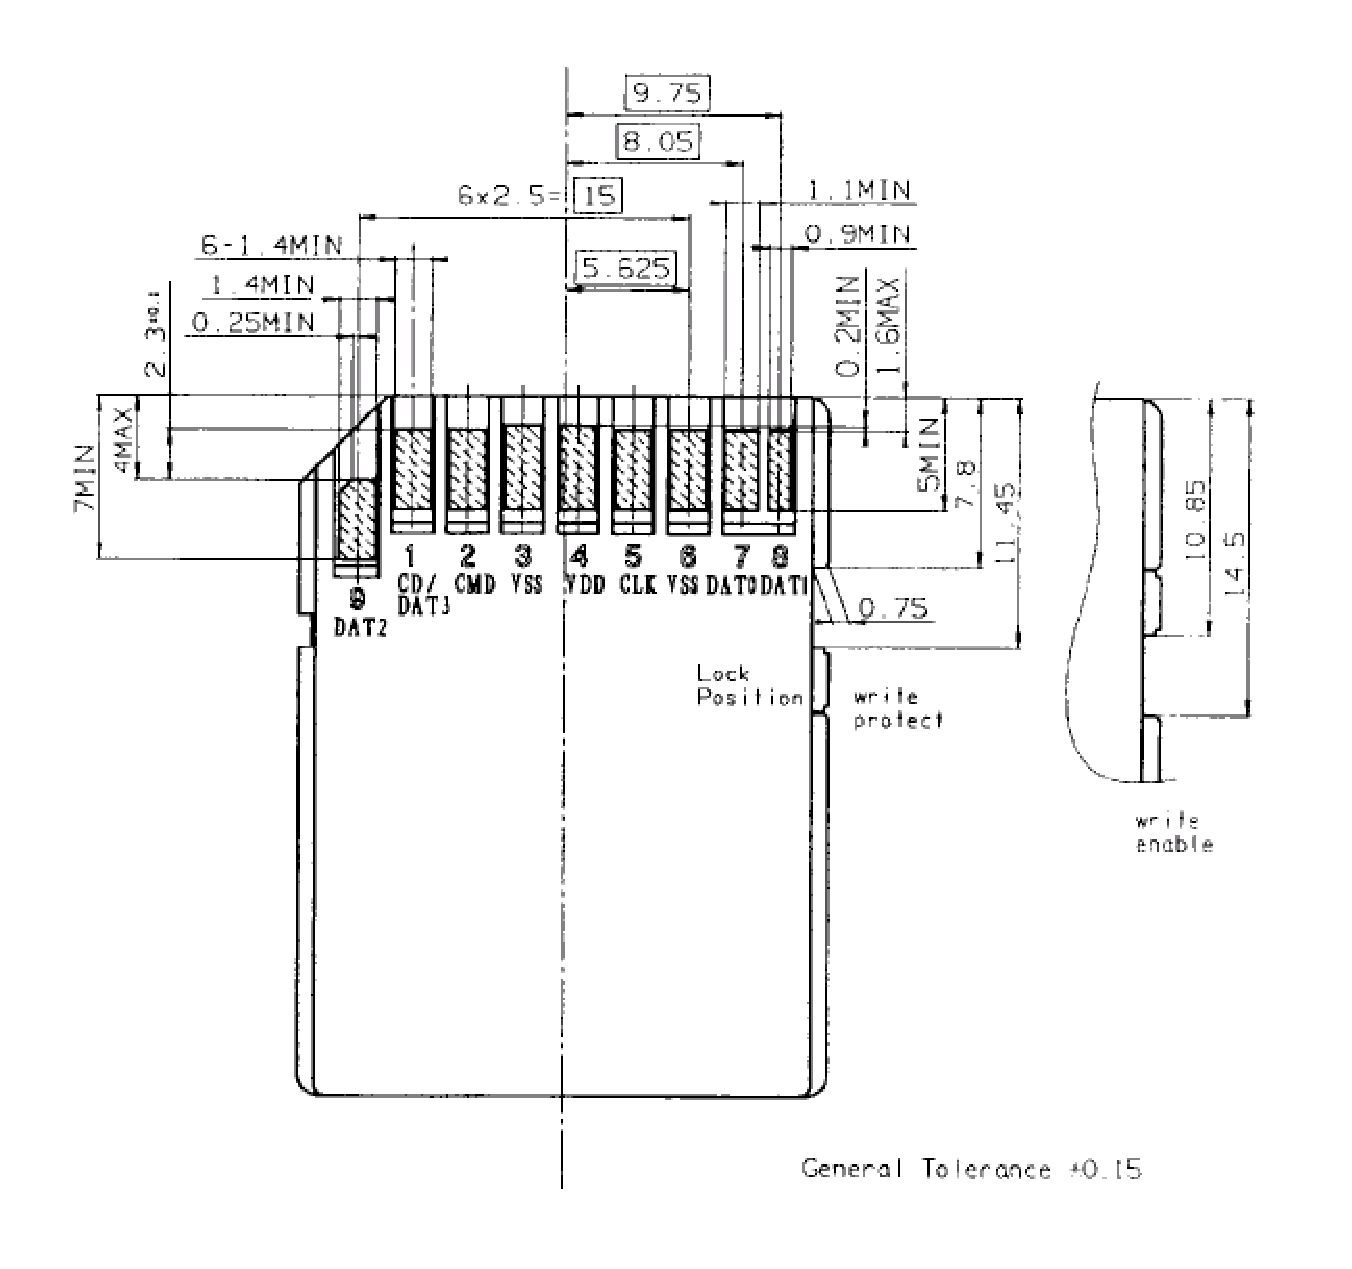
\includegraphics[scale=0.65]{pics/sdcard.eps}
\newline
%\parbox[c]{.4\textwidth}{\begin{center}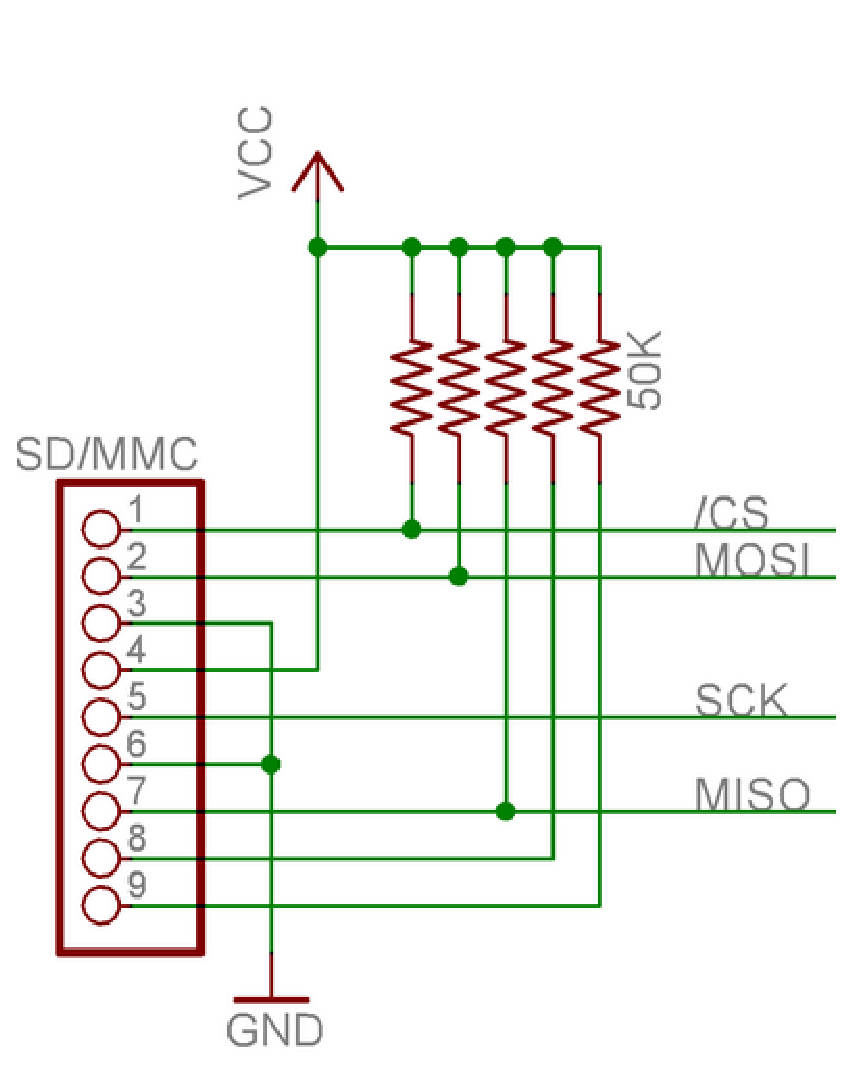
\includegraphics[width=.4\textwidth]{pics/sdconnection}\end{center}}
\parbox[c]{.5\textwidth}{
Connect the following lines on the SD-card:
\begin{itemize}
	\item{Pin 9 (DAT2) - NC\\(or pull-up to 3.3V)}
	\item{Pin 1 (CD) - Any pin on the Atmega128}
	\item{Pin 2 (CMD) - MOSI\\(pin 12 on the Atmega128)}
	\item{Pin 3 (Vss) - GND}
	\item{Pin 4 (Vdd) - +3.3V}
	\item{Pin 5 (CLK) - SCK\\(pin 11 on the Atmega128)}
	\item{Pin 6 (Vss) - GND}
	\item{Pin 7 (DAT0) - MISO\\(pin 12 on the Atmega128)}
	\item{Pin 8 (DAT1) - NC\\(or pull-up to 3.3V)}
\end{itemize}
}
\parbox[c]{.5\textwidth}{\begin{center}
	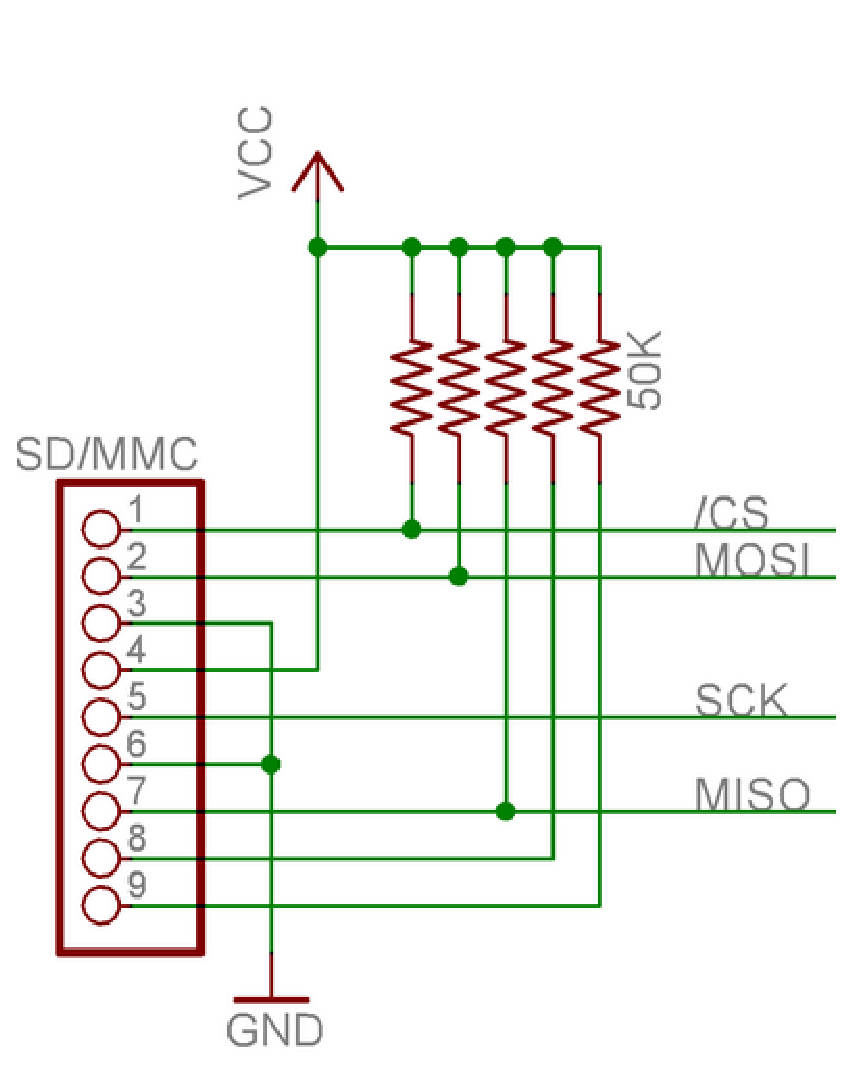
\includegraphics[width=.5\textwidth]{pics/sdconnection}
	\newline\newline
	Remark: this schematic includes pull-up's to 3.3V, which
	can be left off.
\end{center}}
\newline
Remark 1: Make sure that your $\mu C$ is running on 3,3V, so you don't
damage your SD-Card.\newline
\newline
Remark 2: CD is currently static set to PB0, but will become variable
in future releases.
\subsubsection{Download \& Compile}
Let's get started:
\begin{enumerate}
	\item{Get the latest release of efsl on http://www.sf.net/projects/efsl/}
	\item{Unpack the library (on Windows, you can use WinACE or WinRAR)}
	\item{Copy \filename{Makefile-AVR} to \filename{Makefile}}
	\item{Copy \filename{conf/config-sample-avr.h} to \filename{conf/config.h}}
	\item{Compile the library (\code{make lib})}
\end{enumerate}
Now you should have \filename{libefsl.a} in the efsl directory.
\subsubsection{Example}
Since Efsl itself is only a library, it's not supposed to do anything out of 
the box, than just compile. To get started, we'll show here a small example
program that opens an existing file and writes the content to a new file.
\newline\newline
First, create a new directory in which you put the compiled efsl-library 
(\filename{libefsl.a}) and create a new file called \filename{avrtest.c} containing:
\lstset{numbers=left, stepnumber=1, numberstyle=\small, numbersep=5pt, tabsize=4}
\begin{lstlisting}
	#include <efs.h>

	void hang(void);

	void main(void)
	{
		EmbeddedFileSystem efs;
		EmbeddedFile file_r, file_w;
		unsigned short i,e;
		char buf[512];

		if(efs_init(&efs,0)!=0){
			hang();
		}

		if(file_fopen(&file_r,&efs.myFs,"orig.txt",'r')!=0){
			hang();
		}

		if(file_fopen(&file_w,&efs.myFs,"copy.txt",'w')!=0){
			hang();
		}

		while(e=file_read(&file_r,512,buf)){
			file_write(&file_w,e,buf);
		}

		file_fclose(&file_r);
		file_fclose(&file_w);

		fs_umount(&efs.myFs);

		hang();
	}

	void hang(void)
	{
		while((1))
			_NOP();
	}
\end{lstlisting}
$ $\newline
Some extra information on the code above:
\begin{itemize}
	\item{Line 1: The header file for efsl is included here. When using the
		basic efsl functions, \filename{efs.h} is the only header file on the 
		efsl library that needs to be included.}
	\item{Line 7: The object efs is created, this object will contain
		information about the hardware layer, the partition table and
		the disc.}
	\item{Line 8: The objects \code{file\_r} and \code{file\_w} are created, these objects 
		will contain information about the files that we will open on the 
		efs-object.}
	\item{Line 9: A buffer of 512 bytes is allocated. This buffer will be
		used for reading and writing blocks of data.}
	\item{Line 12: Call of \code{efs\_init()}, which will initialize the efs-object.
		To this function we pass:
		\begin{enumerate}
			\item{A pointer to the efs-object.}
			\item{A pointer to the file that contains the partition table /
				file system (in this example, we select a device as file).}
		\end{enumerate}
		If this function returns 0, it means that a valid fat partition is
		found on the SD-card connected.
		If no valid fat-filesystem is found, or the file does not exist, the
		function returns a negative value. In this example we then go to an
		infinite loop to prevent the program to continue.}
	\item{Line 16 \& 20: Call of \code{file\_fopen()}, which will initialize the
		file-objects. To this function we pass:
		\begin{enumerate}
			\item{A pointer to the file-object.}
			\item{A pointer to the filesystem-object.}
			\item{A pointer to the filename.}
			\item{A char containing the the mode (read, write, append).}
		\end{enumerate}
		If this function returns 0, it means the file has successfully been
		opened for reading / writing / appending.
	 	If the file could not be opened (because for example a file already 
		exists), a negative value is returned.}
	\item{Line 24: Call of \code{file\_read()}, which will read a given value of
		bytes (in this example 512) from a file and put it's content into
		the buffer passed (in this example called buf). This function returns
		the amount of bytes read, so the while-loop will be executed as long
		as there are bytes left in the file.}
	\item{Line 25: Call of \code{file\_write()}, which will write a given value
		of bytes (in this example, the amount of bytes that was read
		by \code{file\_read()}) from the buffer passed to a file. This function returns
		the amount of bytes written.}
	\item{Line 28 \& 29: Call of \code{file\_fclose()}, which will close the
		file-objects.}
	\item{Line 31: Call of \code{fs\_umount()}, which will write all buffers to
		the the SD-card.}
\end{itemize}
\subsubsection{Testing}
So now let's test the program:
\begin{enumerate}
	\item
	{
		Make sure that your directory contains both the example from above
		called \filename{avrtest.c} and the library \filename{libefsl.a}.
	}
	\item
	{	Compile the program:
		\begin{itemize}
			\item{On Linux (with avr-gcc): avr-gcc -I/home/user/efsl/inc/ 
				-I/home/user/efsl/conf -ffreestanding -mmcu=atmega128 -Os -o 
				avrtest.o avrtest.c -L./ -lefsl}
			\item{On Windows (with WinAVR): avr-gcc 
				-Ic:$\backslash$efsl$\backslash$inc
				-Ic:$\backslash$efsl$\backslash$conf 
				-ffreestanding -mmcu=atmega128 -Os -o
				avrtest.o avrtest.c -L.$\backslash$ -lefsl}
		\end{itemize}
	}
	\item{Generate a hexfile 
		(avr-objcopy -j .text -j .data -O ihex avrtest.o avrtest.hex)}
	\item{Connect an SD-card to your Atmega128 with a file called 
		\filename{orig.txt} on it.}
	\item
	{
		Flash the hex file into your $\mu C$.
		\begin{itemize}
			\item{On Linux: avrdude -P /dev/ttyUSB0 -c stk500 -p m128 -Uflash:w:avrtest.hex}
			\item{On Windows: use Atmel AVR-Studio}
		\end{itemize}
	}
	\item{Reset your $\mu C$ and wait some time (depending on how big
		the file \filename{orig.txt} is).}
	\item{Disconnect the SD-card, so you can put it in your card reader
		and find out if the file \filename{orig.txt} is copied to 
		\filename{copy.txt}.}
\end{enumerate}
